%%%%%%%%%%%%%%%%%%%%%%%%%%%%%%%%%%%%%%%%%%%%%%%%%%%%%%%%%%%%%%%%%%%%%%%%%%%%
%% PHOTOIONISATION
%%%%%%%%%%%%%%%%%%%%%%%%%%%%%%%%%%%%%%%%%%%%%%%%%%%%%%%%%%%%%%%%%%%%%%%%%%%%

\section{Computing $\mbox{\boldmath $f''(\omega)$ } $}
From equation~\ref{eq:fpp-sigma} we see that in order to determine the imaginary
component of the anomalous form factor $f''$ we need to know the total
photoionisation cross section. Therefore the basic tool that is required is the
computation of the photo-electric matrix element which will give as the
photoionisation amplitude. This matrix element can then be used in two
approaches to computing $f''$ such as:
\begin{itemize}
    \item Relativistic First Order Perturbation Theory
    \item Second Order S-Matrix Theory
\end{itemize}
We have concentrated on obtaining results for the form factor
using second order S-Matrix theory.
The purpose is to attempt to obtain analytic solutions to these problems.
Numerical techniques will be used when it is no longer possible to solve a
problem analytically.

\section{Amplitude for Photoionisation}
The relativistic photon absorption and emission operators for many electron atoms are 
defined~\cite{Kissel-S-Matrix} as:
\begin{eqnarray} \label{eq:photon-abs-emis}
    \mathcal{A}_i       & = & \sum_j \Alpha \cdot \hat{\epsilon}_j \Exp{k_i}{r_j} \\
    \mathcal{A}_f^{\dag}   & = & \sum_j \Alpha \cdot \hat{\epsilon}_j \ExpM{k_f}{r_j}
\end{eqnarray}
where the sum is over all the electrons in an atom, $\Alpha$ is the Dirac alpha
matrix, $\mb{r_j}$ is the position of the $j$-th electron, $\hat{\epsilon}_j$ is 
the polarisation of the photon and $\mb{k}$ is the wave vector of the photon.
The subscripts $i$ and $f$ indicate initial and final states respectively. This
is needed if we are considering for example Compton (inelastic) scattering where
the momentum of the photon changes in a scattering process. However, for the
case of Rayleigh scattering the photon momentum is unchanged 
($\hbar \omega_i = \hbar \omega_f$) and as such in this case we drop the
subscripts and just use the symbols $\omega$ and $\mb{k}$.
\begin{figure}[h]
    \begin{center}
        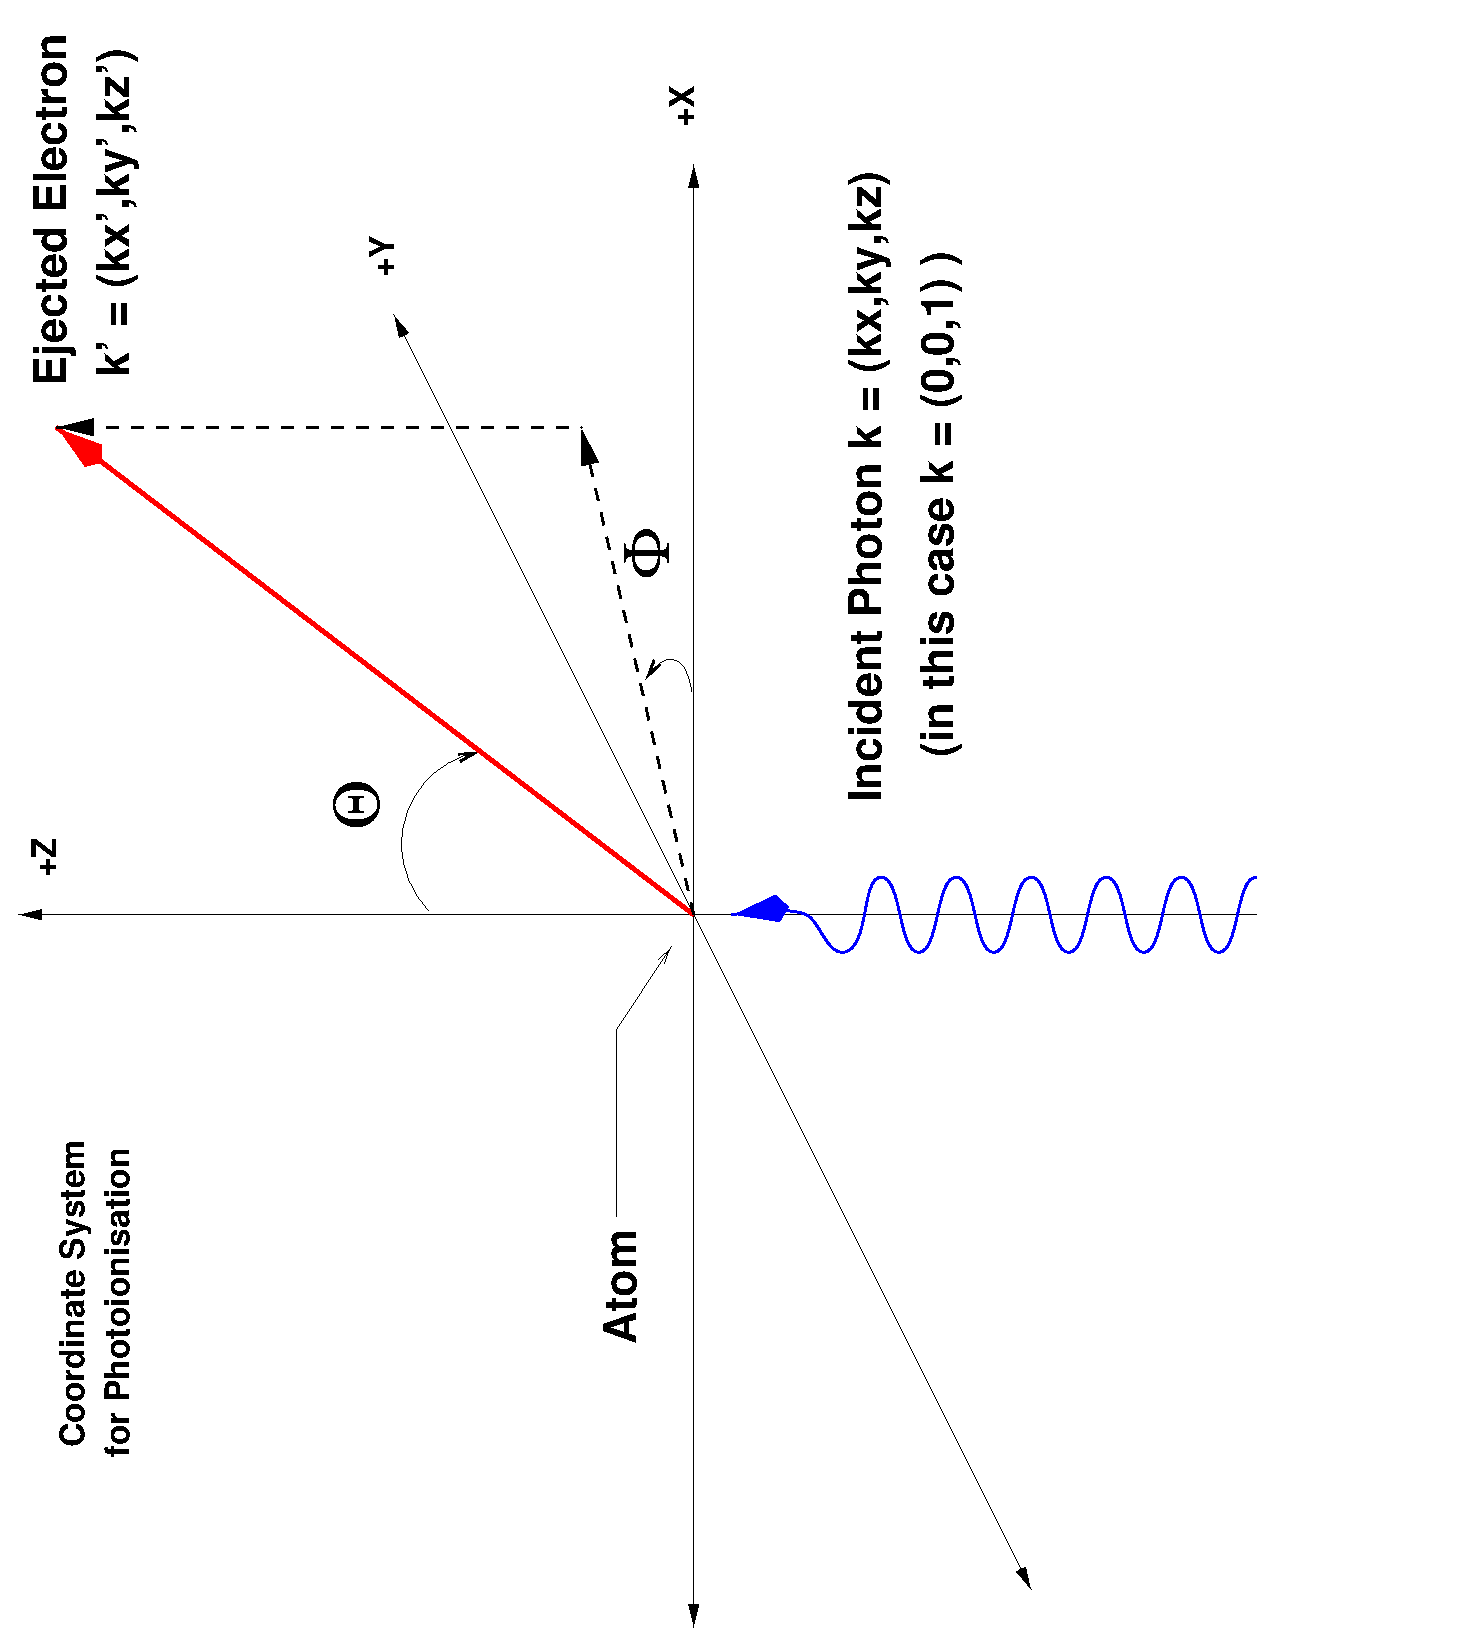
\includegraphics[angle=-90,width=7cm]{coords.eps}
    \end{center}
    \caption{Coordinate System for Photoionisation~\cite{Bransden-Joachain}}
    \label{fig:coordinates}
\end{figure}

We also need to define the coordinate system to be used to describe
photoionisation. The coordinate system setup is shown in figure~\ref{fig:coordinates}.
The small case angles $(\theta,\phi)$ are used to describe the
angular position of an electron bound to an atom, whereas the angles
$(\Theta,\Phi)$ are used to describe the electron ejected angle.
We make the following assumptions:
\begin{itemize}
    \item The incident photon has energy $\hbar \omega$ and is traveling
          in the $+Z$ direction with a momentum wave-vector 
          $\mb{k} = (k_x,k_y,k_z)$.
    \item The photon has a constant well defined polarisation. We will consider photon
          polarisations in the $x$ and $y$ directions. 
    \item The ejected electron has a wave-vector $\mb{k'} = {k'_x,k'_y,k'_y}$
          which defines its linear momentum and ejection direction/angles since:
          \begin{equation} \label{eq:ejection-angles}
          \begin{array}{cccc}
            k'_x & = & |k'| \sin(\Theta) \cos(\Phi) & \\
            k'_y & = & |k'| \sin(\Theta) \sin(\Phi) & \\
            k'_z & = & |k'| \cos(\Theta)&
          \end{array}
          \end{equation}
    \item The atom is initially in it's ground state, and is represented by a 
          $\ket{1S_{1/2}}$ (or $\ket{0}$ or $\psi_0$) wave-function 
          (non relativistic or relativistic).
    \item After photoionisation the ejected electron will be represented by a
          continuum (or free electron) state $\ket{c}$ (or $\psi_c$), 
          (non relativistic or relativistic).
\end{itemize}


\subsection{Photoionisation to a Continuum State}
    We first consider the first order photo-electric matrix element for a single
    electron atom using~\ref{eq:photon-abs-emis}:
    \(
        A_1 = \bra{\psi_c} \mathcal{A} \ket{\psi_0} = \bra{\psi_c} \Exp{k}{r} \Alpha_j \ket{\psi_0} .
    \)
    In the case that the incident photon is polarised either in the $x$ or $y$
    direction, and knowing that the second components of the ground state
    and continuum states are both zero ($\psi_{02} = 0$ and $\psi_{c2} = 0$)
    results in the following form for $A_1$:
    \[ 
        A_1 = \bra{\psi_c} \Exp{k}{r} \Alpha_j \ket{\psi_0} =
        \left\{ 
        \begin{array}{llllll} 

            \int \state{c}{1}^{*} \Exp{k}{r} \state{0}{4} \; d^3 \mb{r} 
            & + &
            \int \state{c}{4}^{*} \Exp{k}{r} \state{0}{1} \; d^3 \mb{r}
            & = & m_1 + m_2
            & \mbox{, if $j = x$} 

            \\[3mm]

            -i \int \state{c}{1}^{*} \Exp{k}{r} \state{0}{4} \; d^3 \mb{r}
            & + &
             i \int \state{c}{4}^{*} \Exp{k}{r} \state{0}{1} \; d^3 \mb{r}
            & = & -i m_1 + i m_2
            & \mbox{, if $j = y$} 

        \end{array} 
        \right .
    \]
    With known values for the spinor components $\state{c}{1}$, $\state{c}{4}$,
    $\state{0}{1}$ and $\state{0}{4}$ we can determine the integrals $m_1$ and
    $m_2$.

    With $\state{c}{1}^{*} = \ExpM{k'}{r}$ and 
    $\state{0}{4} = -i\sqrt{\frac{2}{3}} Y_{11}(\theta,\phi) f_0(r)
                  =  \frac{i}{\sqrt{4 \pi}} \sin(\theta) e^{i \phi} f_0(r)$
    we obtain for the $m_1$ integral:
    \[
    m_1 = \frac{i}{\sqrt{4\pi}} \int \sin(\theta) 
          e^{i \phi} \Exp{k}{r} \ExpM{k'}{r} f_0(r) \; d^3 \mb{r}
    \]
    To do the integration we change to spherical polar coordinates,
    $\mb{r} = r (\sin\phi \cos\theta,\sin\phi \sin\theta, \cos\phi)$, and we
    define 
    \begin{equation}
        \Muq = q_x \sin\phi \cos\theta + 
               q_y \sin\phi \sin\theta +
               q_z \cos\phi
    \end{equation}
    where $\mb{q} = \mb{k} - \mb{k'} = (q_x,q_y,q_z)$.
    Using the definition of $\Muq$ and using 
    $f_0(r) = F_0 G_0 r^{\gamma_1 - 1} e^{-\frac{1}{2}\sigma_1 r}$, $m_1$
becomes:
    \[
    m_1 = F_0 G_0 \frac{i}{\sqrt{4\pi}} \int
          \sin(\theta) e^{i\phi} e^{i\Muq} r^{\gamma_1 - 1} 
          e^{-\frac{1}{2}\sigma_1 r} \; d^3 \mb{r}
    \]
    We can now convert the integral over all space into one using spherical
    polar coordinates.
    \[
    m_1 = F_0 G_0 \frac{i}{\sqrt{4\pi}}
          \int_{0}^{2\pi}
          \int_{0}^{\pi}
          \int_{0}^{\infty}
            \sin^2(\theta) e^{i\phi} r^{\gamma_1 + 1}
            e^{-[ \frac{1}{2}\sigma_1 - i \Muq ] r }
          \; dr \; d\theta \; d\phi
    \]
    The angular integrations over $\theta$ and $\phi$ cannot be solved
    analytically due to the fact that $\Muq$ is a non simple function 
    of $\theta$ and $\phi$. However, using the fact that
    \(
        \int_0^\infty e^{-ax} dx = \Gamma(n+1)/a^{n+1}
    \)
    the radial integral can be solved.
    \[
    m_1 = \frac{i}{\sqrt{4\pi}} F_0 G_0 \Gamma(\gamma_1 + 2)
          \int_{0}^{2\pi}
          \int_{0}^{\pi}
            \left[
                \frac{\sin^2(\theta) e^{i\phi} }{
                    \left(
                        \frac{1}{2} \sigma_1 - i \Muq
                    \right)^{\gamma_1 + 2}
                }
            \right]
          \; d\theta
          \; d\phi
    \]

    We can determine the integral $m_2$ following a similar process to that used
    to determine $m_1$. In the case of $m_2$ the spinor components are given by
    $\state{c}{4}^{*} = \xi(k'_x - ik'_y)\ExpM{k'}{r}$ and 
    $\state{0}{1} = Y_{00}g_0(r) 
                  = \frac{1}{\sqrt{4\pi}} G_0
                     e^{-\frac{1}{2}\sigma_1 r} r^{\gamma_1 - 1}$
    we obtain for $m_2$:
    \[
    m_2 = \frac{\xi(k'_x -ik'_y)}{\sqrt{4\pi}} G_0 \Gamma(\gamma_1 + 2)
          \int_{0}^{2\pi}
          \int_{0}^{\pi}
            \left[
                \frac{\sin(\theta) }{
                    \left(
                        \frac{1}{2} \sigma_1 - i \Muq
                    \right)^{\gamma_1 + 2}
                }
            \right]
          \; d\theta
          \; d\phi
    \]
    
    Using $m_1$ and $m_2$ we can obtain an equation for the first order
    photo-electric amplitude $A_1(\mb{k},\mb{k'})_j$, where $j$ denotes 
    the polarisation direction.

        % X DIRECTION

    \begin{equation} \label{eq:A1-X}
    \boxed{
    A_1(\mb{k},\mb{k'})_x =
    \frac{G_0 \Gamma(\gamma_1 + 2)}{\sqrt{4\pi}}
    \int_{0}^{2\pi}
    \int_{0}^{\pi}
        \left[
            \frac {
            \sin(\theta) [ \xi(k'_x - ik'_y) + i F_0 \sin(\theta) e^{i\phi} ]
%                i F_0 \sin^2(\theta) e^{i\phi} + \xi(k'_x - ik'_y)\sin(\theta)
            } {
                (\frac{1}{2}\sigma_1 - i \Muq )^{\gamma_1 + 2}
            }
       \right]
    \; d\theta
    \; d\phi
    }
    \end{equation}

        % Y DIRECTION

    \begin{equation} \label{eq:A1-Y}
    \boxed{
    A_1(\mb{k},\mb{k'})_y =
    \frac{G_0 \Gamma(\gamma_1 + 2)}{\sqrt{4\pi}}
    \int_{0}^{2\pi}
    \int_{0}^{\pi}
        \left[
            \frac
            {
            i \sin(\theta) [ \xi(k'_x - ik'_y) - i F_0 \sin(\theta) e^{i\phi} ]
%                F_0 \sin^2(\theta) e^{i\phi} + \xi(k'_y + ik'_x)\sin(\theta)
            } {
                (\frac{1}{2}\sigma_1 - i \Muq )^{\gamma_1 + 2}
            }
        \right]
    \; d\theta
    \; d\phi 
    }
    \end{equation}
    These results have been derived without any approximations to the plane wave
    form of the electromagnetic field ($\Exp{k}{r}$) in the absorption and
    emission operators. This is the ``all poles'' approach. 
    In the electric dipole (E1) approximation we have $\Exp{k}{r} \approx 1$.
    We can interpret this as having no information about the propagation
    direction of the incident photon and hence in the electric dipole
    approximation $\mb{k} = 0$.
    Therefore to obtain results for the electric dipole approximation from
    equations~\ref{eq:A1-X} and~\ref{eq:A1-Y} it is simply a matter of
    setting $\mb{k} = 0$.
    \begin{equation} \label{eq:A1-Dipole}
    \boxed{
        A_1^{E1}(\mb{k},\mb{k'})_j = A_1(0,\mb{k'})_j
    }
    \end{equation}

\subsection{Photoionisation in the Forward Scattering Direction}
The integrals $m_1$ and $m_2$ defined in the previous section cannot be solved
analytically in general. However, it is possible to obtain an analytic solution 
for some special cases. One such case is when the incident photon is traveling
in the $+z$-direction with a propagation vector $k\hat{\mb{n}} = (0,0,k)$ and 
the electron is ejected in the $\Theta = 0$ (or forward scattering direction).
In this case, the propagation vector for the ejected electron is
$k'\hat{\mb{n}}' = (0,0,k')$.

We note from these assumptions that the integral $m_2 = 0$ because it is 
multiplied by the factor $\xi (k_x' - i k_y')$ and in the forward scattering
direction $k_x' = 0$ and $k_y' = 0$. We also note that the the function $\Muq$
is simplified to $\Muq = q_z \cos(\theta)$. We these new assumption we can 
rewrite the integral for $m_1$ and attempt an analytic solution.
\[
    m_1 = \frac{i}{\sqrt{4\pi}}
    \int_{0}^{\infty}
    \int_{0}^{2\pi}
    \int_{0}^{\pi}
        \sin^2(\theta) e^{iq_z \cos(\theta)} e^{i\phi} r^2 f_0(r) 
    \; d\theta
    \; d\phi
    \; dr
\]
Integrating over $\phi$ gives $2i$ and making use of the trigonometric
identity $2\sin^2(\theta) = 1-\cos(\theta)$, $m_1$ can be written as:
\begin{eqnarray*}
    m_1 & = & \frac{-2}{\sqrt{4\pi}}
    \int_0^\infty
        f_0(r) r^2
        \left[
            \frac{1}{2} 
            \int_0^\pi
                e^{i q_z r \cos(\theta) }
            \; d\theta
            +
            \frac{1}{2}
            \int_0^\pi
                \cos(2\theta) e^{i q_z r \cos(\theta) }
            \; d\theta
        \right]
    \; dr 
    \\
    & = &
    \frac{-2}{\sqrt{4\pi}}
    \int_0^\infty
    f_0(r) r^2
    \left[
        \frac{1}{2} ( \pi J_0(q_z r)  +  \pi J_2(q_z r) )
    \right]
    \; dr
    \\
    & = &
    \frac{-\pi F_0 G_0}{\sqrt{4\pi}}
    \left[
        \int_0^\infty
            J_0(q_z r) r^{\gamma_1 + 1} e^{-\frac{1}{2} \sigma_1 r}
        \; dr
        +
        \int_0^\infty
            J_2(q_z r) r^{\gamma_1 + 1} e^{-\frac{1}{2} \sigma_1 r}
        \; dr
    \right]
\end{eqnarray*}
where $J_n(x)$ is a Bessel function of the first kind of order $n$.
The integrals involving the Bessel functions can be solved in terms of the
hypergeometric function $_2 F_1(a,b;c;z)$~\footnote{These integrals were solved
using Mathematica 3.0}. Since $m_2$ is zero, the first order amplitude is given
in terms of $m_1$, where we have $A(k,k')_x = m_1$ and $A(k,k')_y = -i m_1$, for
photon polarisations in the $x$ and $y$ directions respectively. 
Using this information, and substituting in the for the constants $F_0$, 
$G_0$ and $\sigma_1$ which were defined earlier, the analytic solutions
for the first order photo-electric matrix elements in the forward scattering
direction are given by:
\begin{equation} \label{eq:A1-Forward}
\boxed{
\begin{split}
     A_1 & (k,k')_x  =  \frac{\pi}{\sqrt{\pi}}  
                        \left( \frac{2Z}{a_0} \right)^{3/2}
                        \sqrt{ \frac{1 - \epsilon_1}{
                                    2 \Gamma(2\gamma_1 + 1)
                               } } \times \\
    & \Biggl\{
        \left( \frac{Z}{a_0} \right)^{-(\gamma_1 + 2)}
    \Gamma(\gamma_1 + 2)
    \; _2 F_1 \left(
                \frac{\gamma_1 + 2}{2} ,
                \frac{\gamma_1 + 3}{2} ;
                1 ;
                - \left(
                    \frac{2a_0}{Z}
                \right)^2
                (k - k')^2
           \right)
    + \\ & 
    \frac{1}{8} (k - k')^2 
    \left( \frac{Z}{a_0} \right)^{-(\gamma_1 + 4)}
    \Gamma(\gamma_1 + 4)
    \; _2 F_1 \left(
                \frac{\gamma_1 + 4}{2} ,
                \frac{\gamma_1 + 5}{2} ; 
                1 ;
                - \left( \frac{2a_0}{Z} \right)^2
                (k - k')^2
            \right)
    \Biggr\}
\end{split}
}
\end{equation}
\begin{equation}
\boxed{
    A_1(k,k')_y = -i A_1(k,k')_x
}
\end{equation}
This implies that in the forward scattering direction, the probability of
photoionisation is the same for a photon polarised in the $x$ or $y$ direction,
because \( |A_1(k,k')_x|^2 = |A_1(k,k')_y|^2 \).

%%%%%%%%%%%%%%%%%%%%%%%%%%%%%%%%%%%%%%%%%%%%%%%%%%%%%%%%%%%%%%%%%%%%%%%%%%%%%%%%%%%%%%%%%
% S-MATRIX THEORY
%%%%%%%%%%%%%%%%%%%%%%%%%%%%%%%%%%%%%%%%%%%%%%%%%%%%%%%%%%%%%%%%%%%%%%%%%%%%%%%%%%%%%%%%%
\section{S-Matrix Theory}
S-matrix theory as developed in covariant perturbation theory (or quantum field
theory) is used to solve a large number of scattering problems in quantum
mechanics~\cite{Sakurai-Advanced,Greiner,Yndurain,Akhiezer,Weinberg}.
The use of S-matrix theory to compute atomic form factors has been applied by
Kissel and Pratt~\cite{Kissel-S-Matrix}.
For a given photon of energy $\hbar \omega$ the second order S-matrix (scattering) 
amplitude $A_2(\omega)$ is related to the imaginary component of the form factor 
$f''(\omega)$ and to the total cross section $\sigma^{TOT}(\omega)$ through the
following relation:
\begin{equation}
    \mathrm{Im} A_2(\omega) = r_0 f''(\omega) = \frac{\omega}{4 \pi c} \sigma^{TOT}(\omega)
\end{equation}
The relationship between the total cross section and $f''(\omega)$ is the same
as equation~\ref{eq:fpp-sigma}. Although here we will only be considering the
photoionisation cross section, $\sigma^{TOT}(\omega)$ may also include partial cross
section contributions from other process such as bound-bound transitions. 
In addition to this we also have that:
\begin{itemize}
    \item The second order amplitude considers only the forward scattering direction.\\
          $A_2(\omega) = A_2(\omega,\Theta=0)$.
    \item The sign of $f''$ as define by Kissel and Pratt~\cite{Kissel-S-Matrix} 
          is opposite of that used in the crystallography literature
          $(f''_{Kissel} = -f''_{cl})$. We will follow the convention of the
          crystallography community.
    literature.
\end{itemize}

The second order S-matrix amplitude is defined as follows:
\begin{equation}
     A_2 = 
     -r_0 mc^2 \sum_p
     \left[
     \frac{
        \bra{m} \mathcal{A}_f^\dag \ket{p}
        \bra{p} \mathcal{A}_i \ket{n}
     }{
        E_n - E_p + \hbar\omega_f + i0_+
     }
     +
     \frac{
        \bra{m} \mathcal{A}_i \ket{p}
        \bra{p} \mathcal{A}_f^\dag \ket{n}
     }{
        E_n - E_p - \hbar\omega_i + i0_+
     }
     \right]
\end{equation}
where the state $\ket{\psi}$ is a four component relativistic spinor which
satisfies the Dirac equation (equation~\ref{eq:dirac-equation}). The equation describes a second
order scattering process with the subscript $i$ denoting the initial situation
and $f$ denoting the final situation. The two components correspond to the
processes of photoabsorption followed by photoemission, and photoemission
followed by photoabsorption, as shown in the Feynmann diagrams in 
figure~\ref{fig:feynmann}.
\begin{figure}[h]
    \begin{center}
        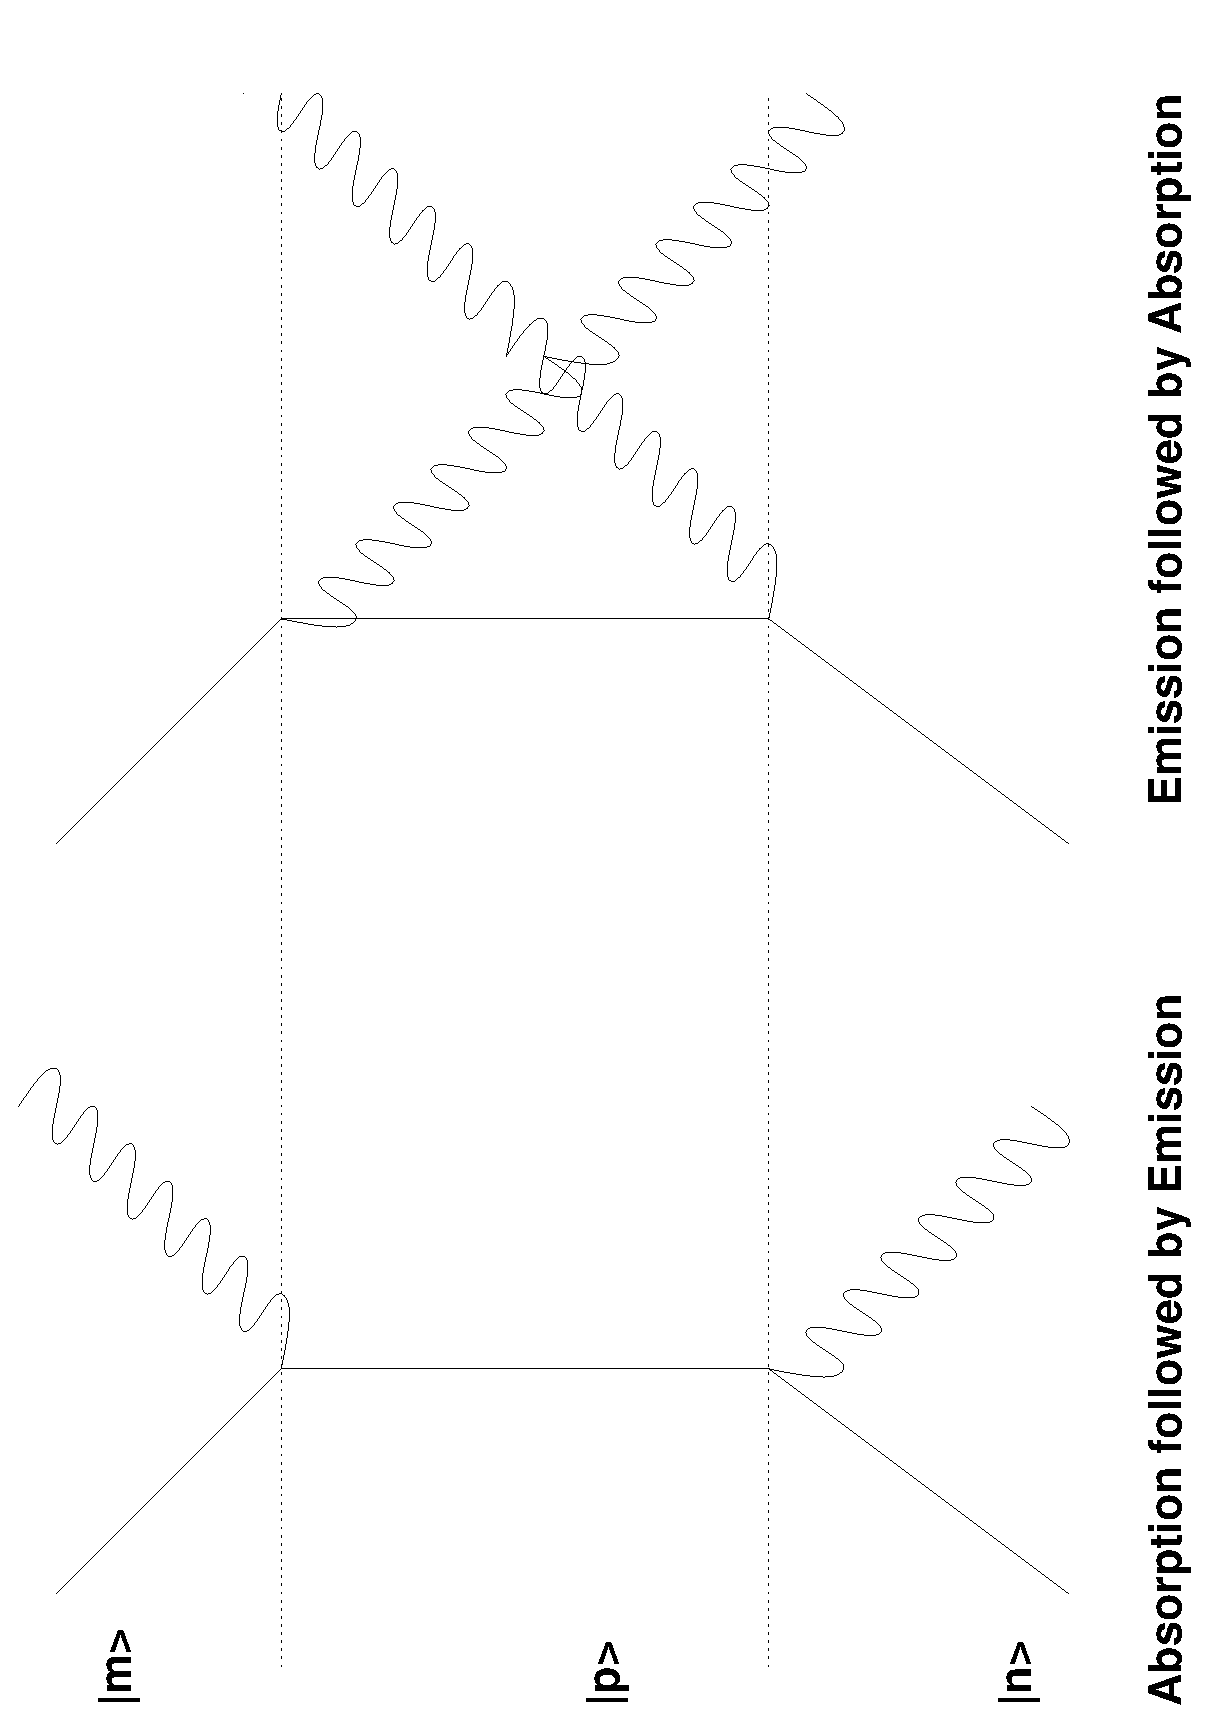
\includegraphics[angle=-90,width=7.0cm]{feynmann.eps}
    \end{center}
    \caption{Second Order Photon Scattering}
    \label{fig:feynmann}
\end{figure}

The initial state of the atom (which we will make
the ground state) is $\ket{n}$, the final state is $\ket{m}$ and we have
a sum of all intermediate states $\ket{p}$. The energy of the initial state is
$E_n$, the energy of the intermediate states is $E_p$, and initial and and final
energy of the photon are $\hbar \omega_i$ and $\hbar \omega_f$ respectively.
The denominator of both components of $A_2(\omega)$ includes a small complex
positive value $i0_+$.

For the case of Rayleigh scattering, 
$\hbar \omega_i = \hbar \omega_f = \hbar \omega$, and the final atomic state is the
same as the the initial atomic state ($\ket{n} = \ket{m}$). 
We can then define the form factor $f''$ in terms of the second order elastic
(Rayleigh) S-matrix $\mathrm{Im}A_2^R(\omega)$.
\begin{equation}
    f''(\omega) = \frac{\mathrm{Im}A_2^R(\omega)}{r_0} 
                = \frac{\omega}{4\pi c r_0} \sigma^{TOT}(\omega)
\end{equation}
If the initial state is the ground state of the hydrogen atom $\ket{\psi_0}$,
and we substitute in for the the emission and absorption operators previously
defined (without the summation since we only have a single electron) we 
obtain:
\begin{equation}
        A_2^R(\omega) = 
        -r_0 mc^2 \sum_p \left[
        \frac{
            \bra{\psi_0} \ExpM{k}{r} \Alpha_j \ket{\psi_p} 
            \bra{\psi_p} \Exp{k}{r}  \Alpha_j \ket{\psi_0}
        }{
            E_0 - E_p + \hbar\omega + i0_+
        } 
     +
        \frac{
           \bra{\psi_0} \Exp{k}{r}   \Alpha_j \ket{\psi_p} 
           \bra{\psi_p} \ExpM{k}{r}  \Alpha_j \ket{\psi_0} 
        }{
           E_0 - E_p - \hbar\omega - i0_+
        }
        \right]
\end{equation}
Making use of 
\(
    \bra{a} X^\dag \ket{b} \bra{b} X \ket{a} 
  = \bra{b} X \ket{a}^* \bra{b} X \ket{a} = | \bra{b} X \ket{a} |^2
\)
and splitting the sum into a sum over discrete states (bound excited states of
the hydrogen atom) and an integral over 
continuum states ($\ket{\psi_c}$ is the free electron continuum state) we obtain:
%\begin{equation}
%\begin{split}
\begin{multline}
    A_2^R(\omega)   =  
         -r_0 mc^2  \int_0^\infty
        \left[
             \frac{
            | \bra{\psi_c} \Exp{k}{r}  \Alpha_j \ket{\psi_0} |^2
        }{
            E_0 - E_c + \hbar\omega + i0_+
        } 
        +
        \frac{
           | \bra{\psi_c} \ExpM{k}{r}  \Alpha_j \ket{\psi_0} |^2
        }{
           E_0 - E_c - \hbar\omega - i0_+
        }
        \right]
        dEc
        \\
         -r_0 mc^2  \sum_p 
        \left[
        \frac{
            | \bra{\psi_p} \Exp{k}{r}  \Alpha_j \ket{\psi_0} |^2
        }{
            E_0 - E_p + \hbar\omega + i0_+
        } 
     +
        \frac{
           | \bra{\psi_p} \ExpM{k}{r}  \Alpha_j \ket{\psi_0} |^2
        }{
           E_0 - E_p - \hbar\omega - i0_+
        }
        \right]
\end{multline}
%\end{split}
%\end{equation}
Ideally both continuum and bound-bound components would be included in
a calculation of the S-matrix amplitude. However, due to time constraints the
calculations focused on the continuum component. From the standard
non relativistic understanding of the photo-electric 
effect~\cite{Sakurai-Modern,Kissel-S-Matrix,Chantler-Book} we know that the 
ground state to continuum amplitude dominates over the bound-bound transition
amplitudes. However Chapter 5 of this report contains some results for
bound-bound, transitions which may be used as a basis for determining 
atomic form factors.

Therefore, we can now write down the second order S-matrix amplitude which needs
be calculated. We see that the matrix elements in the numerators are simply
the first order photoionisation matrix elements 
(equations~\ref{eq:A1-X},~\ref{eq:A1-Y},~\ref{eq:A1-Forward}) so we can write
the second order amplitude in terms of first order amplitudes.
($\omega = kc$).
\begin{equation} \label{eq:A2}
\boxed{
     A_2^R(\omega) = A_2(\mb{k},\mb{k'})_j =
         -r_0 mc^2  
        \left[
        \int_0^\infty
             \frac{
             | A_1(\mb{k},\mb{k'})_j |^2
        }{
            E_0 - E_c + \hbar\omega + i0_+
        } 
        dEc
        +
        \int_0^\infty
        \frac{
            |A_1(\mb{-k},\mb{k'})_j |^2
        }{
           E_0 - E_c - \hbar\omega - i0_+
        }
        dEc
        \right]
}
\end{equation}
The second order amplitude for the electric dipole approximation, 
as for the first order matrix elements is simply given by setting $\mb{k}=0$.
\begin{equation} \label{eq:A2-Dipole}
    \boxed{
       A_2^{E1}(\mb{k},\mb{k'})_j  = A_2(0,\mb{k'})_j  
    }
\end{equation}
\subsection{Computational Method}
To compute $f''$, we need to compute the value of equation~\ref{eq:A2} 
over a range of photon energies ($\hbar \omega$), 
take the imaginary component and then divide by $r_0$.
This was done by developing a computer program in the C++ language to perform 
the computations using
numerical integration methods to solve the integrals in equations~\ref{eq:A1-X}
and~\ref{eq:A1-Y} and the integral over the continuum state (ejected electron
energies).
\begin{itemize}
    \item One of the main computation issues faced was the problem of multi 
          dimensional integrals. Although there was a single outer integral
          over continuum energies to compute the first order matrix element
          required the numerical computation of a two dimensional angular integral.
    \item The integration methods used originally elementary algorithms 
          based on the Simpson's and Trapezoidal rules. The main problem with
          these methods was computation speed and accuracy.
          Performance and accuracy of results improved when the integration
          routines where changed to a 10-point Gauss-Legendre 
          integration method~\cite{Koonin}.
    \item The integration method used for the integral over continuum states
          had to handle integrating over a singularity. This was handled by
          implementing a numerical version of the Cauchy principal value
          technique~\cite{Engineering-Maths}. The integral was split into 
          three regions, below the singularity, near the singularity and
          above the singularity to infinity. The integral to infinity was
          numerically by making an appropriate change of variable, changing
          the integral from one that was over an open interval to one that
          was over a closed interval.
    \item All the computations where done in atomic units (a.u.) 
          giving the standard units of electrons/atom for $f''$.
          The energy axes in keV were converted after the computation
          was performed.
    \item Since $f''(\omega)$ is calculated using the imaginary component
          of the second order S-matrix amplitude the size of the small
          positive complex value $i0_+$ was expected to effect the results.
The pseudo-code below gives an outline of the depth level of all the
numerical integrations involved in the calculation, showing why computation
speed was an issue.
\end{itemize}
 \begin{verbatim} 
    PROGRAM
    {
        For E = Min_Photon_Energy To Max_Photon_Energy With Step=EnergyStep
            Compute 2nd Order Matrix Element
                Integrate A2 Over All Continuum Energies 
                    Compute 1st Order Matrix Element
                        Integrate Over Phi From 0 To 2Pi 
                            Integrate Over Theta From 0 To Pi
    } 
\end{verbatim}


\subsection{Results for $f''(\omega)$ and
            Possible Problems With S-Matrix Theory as Currently Implemented}
Figure~\ref{fig:compare-poles} shows a logplot the form factor ($\log_{10}(f'')$)
for a range of photon energies to 100 keV. The plot compares the result obtained
using the all poles approach with that obtained for $f''$ using the electric
dipole approximation. As can be seen, the all pole and electric dipole approach
are closer in agreement at lower energies. We expect that the electric dipole
approximation breaks down the higher the photon energy we have and this is
indeed the case in the results obtained. This is because the electric dipole
approximation makes the assumption that the wavelength of the photon is much
larger than the size of the atom it is interacting with. At higher energies,
and hence shorter wavelengths, this approximation begins to break down as
is evident in figure~\ref{fig:compare-poles}.
\begin{figure}[h]
\begin{center}
    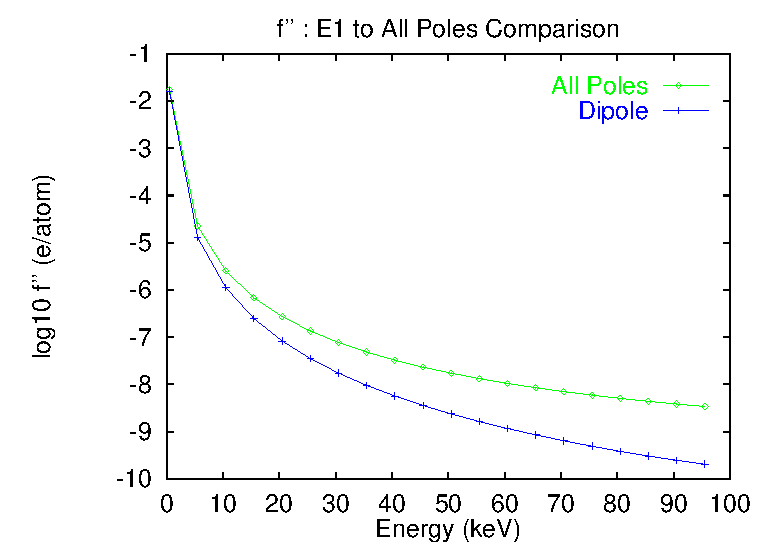
\includegraphics[width=7cm]{compare_poles_1.eps}
\end{center}
    \caption{Relativistic Form Factor $f''$ -- Comparing Electric Dipole 
            to All Poles Result}
    \label{fig:compare-poles}
\end{figure}
\begin{figure}[h]
\begin{center}
    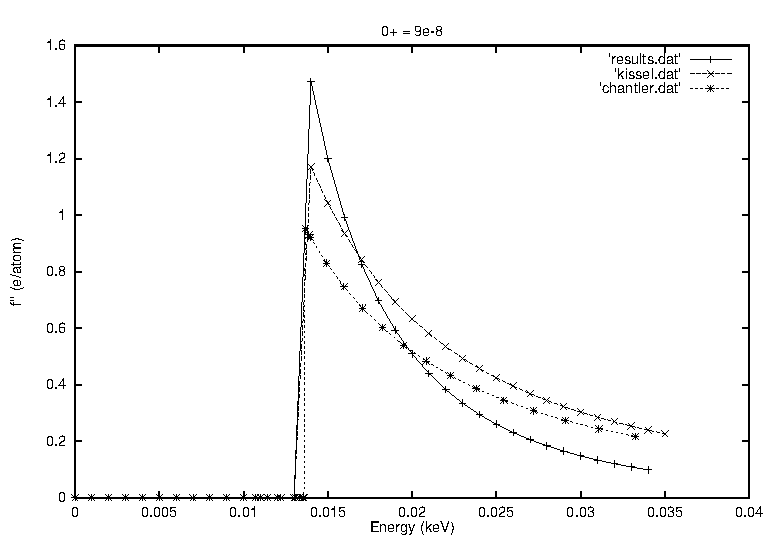
\includegraphics[width=7cm]{compare_fpp_1.eps}
    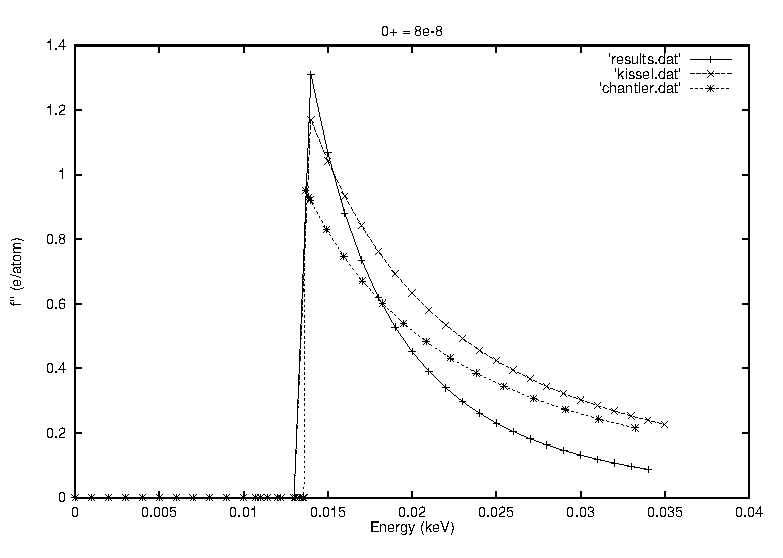
\includegraphics[width=7cm]{compare_fpp_2.eps}
    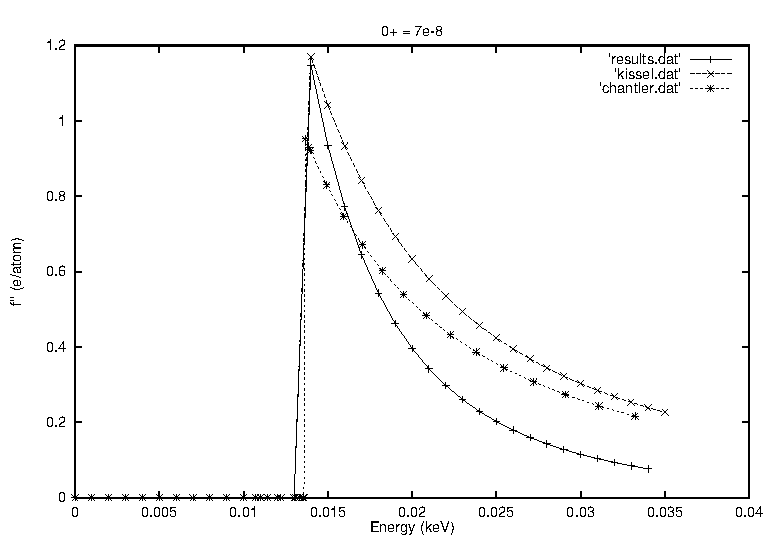
\includegraphics[width=7cm]{compare_fpp_3.eps}
    \caption{Comparing Current Results for $f''$ with those of Chantler
             and those of Kissel and Pratt}
    \label{fig:fpp-compare}
\end{center} 
\end{figure}
Figure~\ref{fig:fpp-compare} shows three plots of $f''(\omega)$ at an energy
range encompassing an edge (in this case the ionisation energy of the hydrogen
atom $E_0 = 13.6$ eV. The plots contain comparisons between these new results,
the S-matrix results of Kissel and Pratt~\cite{Kissel-S-Matrix}, and
the recent results of Chantler~\cite{Chantler-Tabulation}. 
The three plots show the new results for three different values of the
small complex value $i0_+ = 7\times 10^{-8},8\times 10^{-8},9\times 10^{-8}$.
Clearly, the results are affected by the change in size of $i0_+$.
All three theories predict the correct edge at 13.6 eV, all qualitatively
have a similar shape, but there is disagreement between all three.

With regards to the new results, there clearly are some issues that need
to be addressed. The main one is the dependence on $i0_+$. One way to attempt
to solve this problem would be to try to change the integration scheme used 
from a non-convergent method (Gauss-Legendre) used to obtain the current results
to a method such as a form of Romberg integration which converges to a result.
This may or may not fix the problem with regard to the size of $i0_+$.
If the problem still persists, then it could possibly suggest there are still
some problems with S-matrix theory as currently implemented in the area of
calculating atomic form factors.

\subsection{Results for Angular Dependence}
The mod-squared of the second order S-matrix element $|A_2(\mb{k},\mb{k'})_j|$
cannot also be used to study the angular distribution of the ejected electron
(or photoelectrons) at selected energies. We keep the direction
of the photon wave-vector the same ($\mb{k} = k(0,0,1)$) as when calculating
$f''$, just changing the magnitude for different photon energies. 
However the ejected electron wave vector is described by the ejection
angles $(\Theta,\Phi)$ (see equation ~\ref{eq:ejection-angles}). 
In the $f''$ case we were interested in the forward scattering direction
so we set $\Theta = 0$. Alternatively, we can set $\Phi = 0$ and vary
$\Theta$ over a range from $0$ to $2 \pi$. 
This gives as an ejected electron angular distribution for all values of $\Theta$ in
the $\Phi = 0$ plane.

\begin{figure}[h]
\begin{center}
\begin{tabular}{cc}
    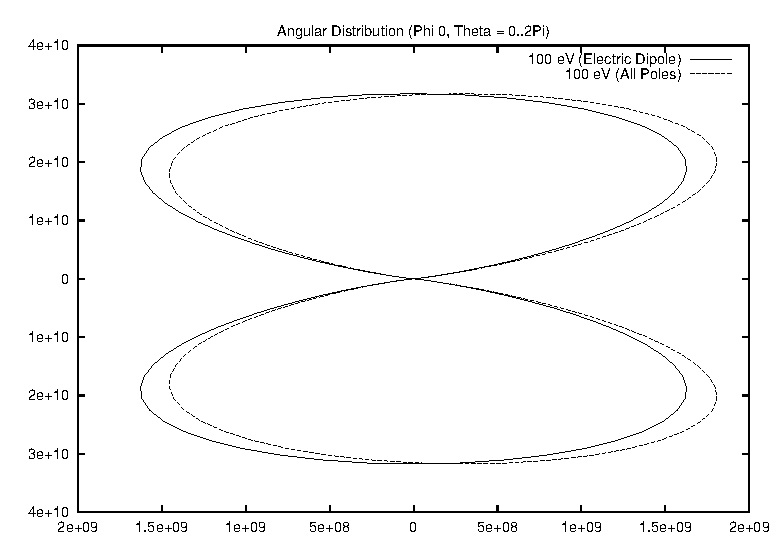
\includegraphics[width=7cm]{ang_100eV_both.eps}
    &
    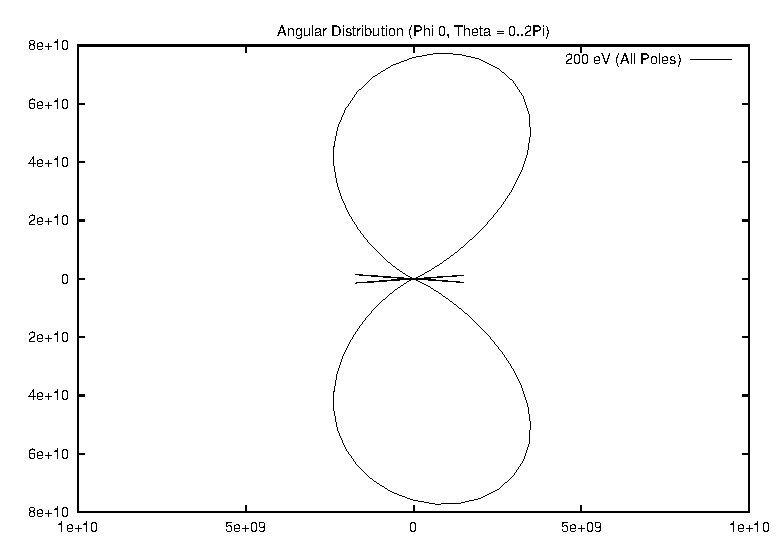
\includegraphics[width=7cm]{ang_200eV_ap.eps}
    \\
    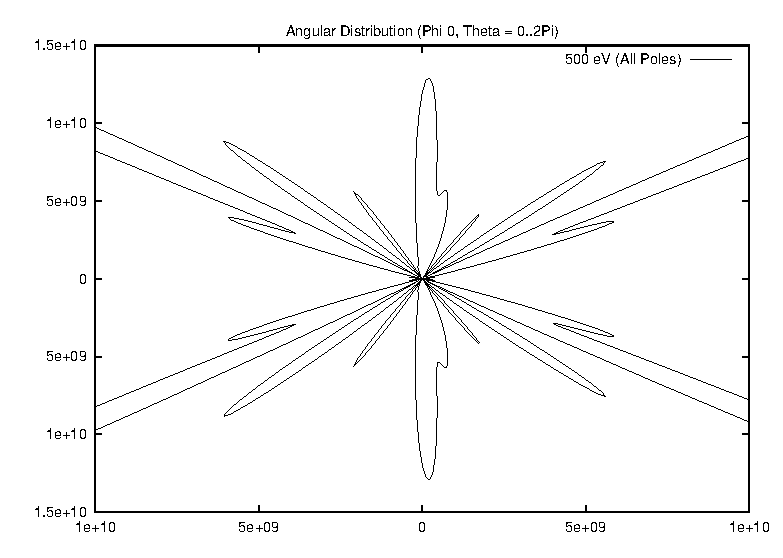
\includegraphics[width=7cm]{ang_500eV_ap.eps}
    &
    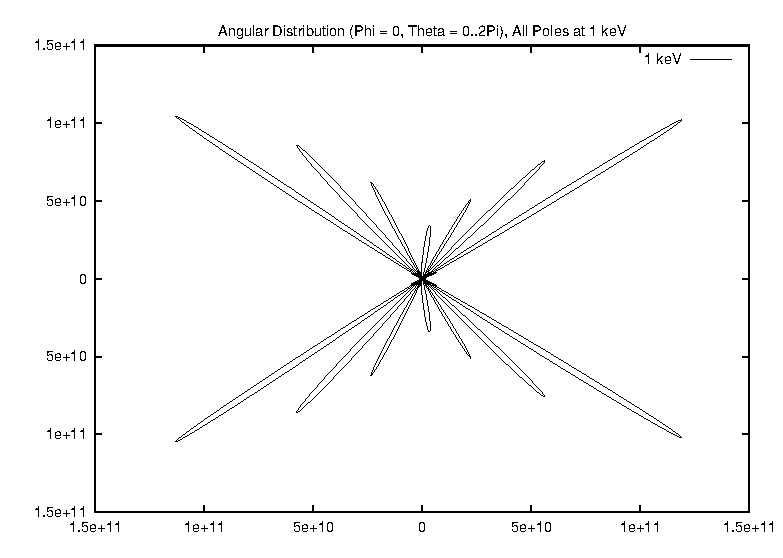
\includegraphics[width=7cm]{ang_1keV_ap.eps}
\end{tabular}
    \caption{Ejected Electron Angular Distributions at Photon Energies of
             100 eV, 200 eV, 500 eV and 1 keV}
    \label{fig:angular-plots}
\end{center}
\end{figure}

The results for $|A_2(\mb{k},\mb{k'})_j|$ at photon energies of
100 eV, 200 eV, 500 eV and 1 keV are shown in figure~\ref{fig:angular-plots}.
The top left plot for a photon energy of 100 eV also shows the distribution
for the electric dipole approximation. 
At the lower energies we see that the plots exhibit a $\sin^2(\Theta)$
distribution. As the energy is increased we see finer definition
of the ejection lobes in all directions, indicating the very precise
directions of electron ejection.


%%%%%%%%%%%%%%%%%%%%%%%%%%%%%%%%%%%%%%%%%%%%%%%%%%%%%%%%%%%%%%%%%%%%%%%%%%%%%%%%%%%%%%%%%
% RELATIVISTIC PERTURBATION THEORY
%%%%%%%%%%%%%%%%%%%%%%%%%%%%%%%%%%%%%%%%%%%%%%%%%%%%%%%%%%%%%%%%%%%%%%%%%%%%%%%%%%%%%%%%%
%\section{Relativistic Perturbation Theory}
%\begin{equation}
%    \frac{d\sigma}{d\Omega} =
%    \frac{\alpha k'}{2 m_e \pi \omega}
%    | \bra{\psi_c} \Exp{k}{r} \Alpha \cdot \hat{\epsilon}_j \ket{\psi_0} |^2
%    = \frac{\alpha k'}{2 m_e \pi \omega} |A_1(k,k')_j|^2 
%\end{equation}

